% !TEX program = xelatex
% Approved input CSV SHA-256: 3bea6823e552063df49fa0bbe03cc830300c6869674c08600baa6b29c046f366
% Decoder: standard; all rates per complete circuit execution.
% Figure captions and benchmark scope are supplied separately.
\documentclass[tikz,border=3pt]{standalone}
\usepackage{fontspec}
\usepackage{unicode-math}
\usepackage{pgfplots}
\usepgfplotslibrary{groupplots}
\defaultfontfeatures{Ligatures=TeX}
\setmainfont{Times New Roman}
\setmathfont{STIX Two Math}
\pgfplotsset{compat=1.18}
\definecolor{deepblue}{HTML}{0000F1}
\definecolor{cyan}{HTML}{00B0FF}
\definecolor{orange}{HTML}{FF9400}
\definecolor{red}{HTML}{F10800}
\begin{document}
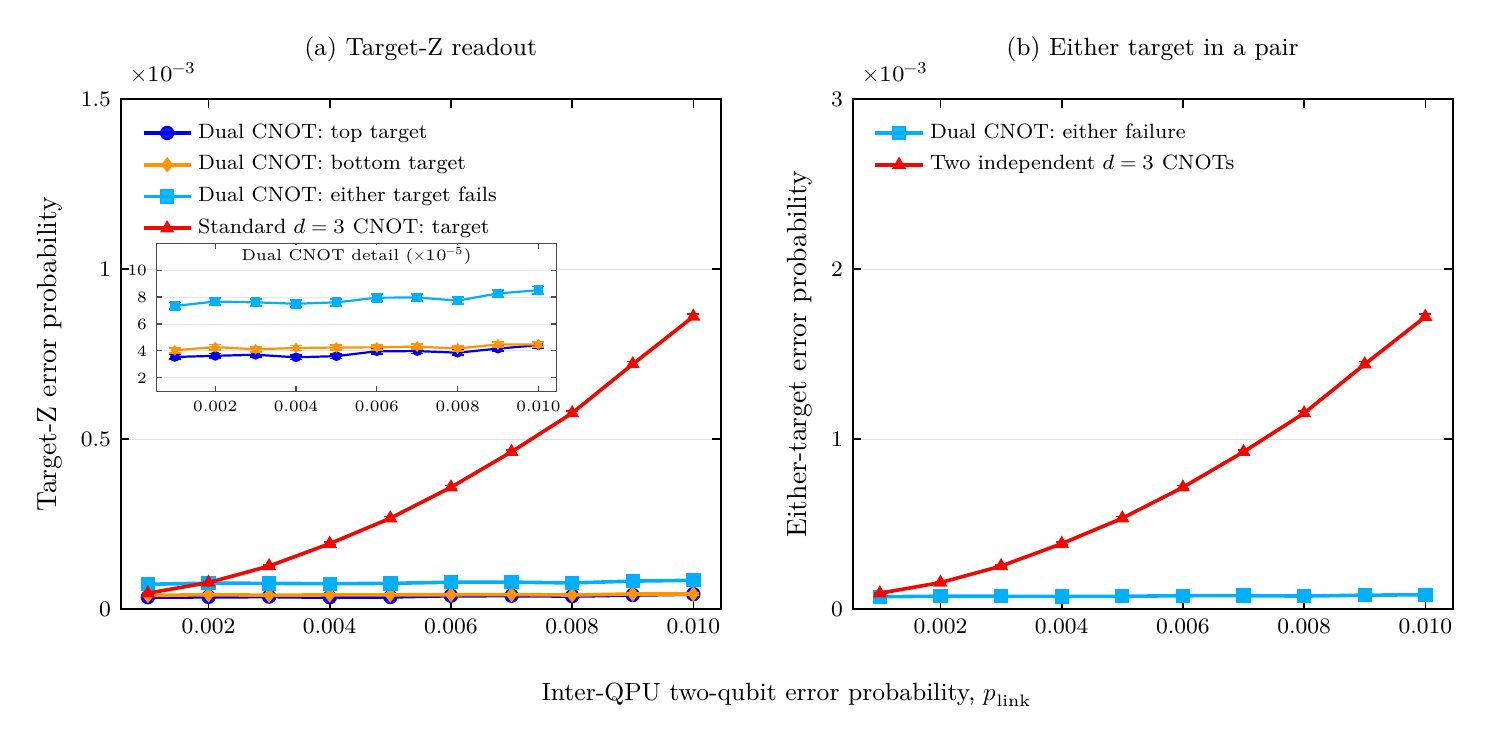
\begin{tikzpicture}
\begin{groupplot}[
group style={group size=2 by 1,horizontal sep=0.66in},
width=3.00in,height=2.55in,scale only axis,
xmin=0.00055,xmax=0.01045,
xtick={0.002,0.004,0.006,0.008,0.010},
xticklabels={0.002,0.004,0.006,0.008,0.010},
scaled ticks=false,
title style={font=\fontsize{9}{10.5}\selectfont,yshift=4pt},
ylabel style={font=\fontsize{9}{10.5}\selectfont},
tick label style={font=\fontsize{8}{9.2}\selectfont},
axis lines=box,tick align=inside,
axis line style={black,line width=0.65pt},
tick style={black,line width=0.60pt},major tick length=3.0pt,
ymajorgrids=true,major grid style={draw=black!13,line width=0.45pt},
clip mode=individual,clip marker paths=false,
legend cell align=left,
legend style={at={(0.025,0.975)},anchor=north west,draw=none,fill=white,fill opacity=0.90,text opacity=1,
font=\fontsize{7.5}{8.7}\selectfont,row sep=0.7pt,inner xsep=2pt,inner ysep=2pt},
]
\nextgroupplot[
title={(a) Target-Z readout},ylabel={Target-Z error probability},
ymin=0,ymax=0.0015,
ytick={0,0.0005,0.001,0.0015},
yticklabels={0,0.5,1,1.5},
extra description/.code={
\node[anchor=south west,font=\fontsize{8}{9.2}\selectfont] at (rel axis cs:0,1.015) {$\times10^{-3}$};
},
]
\addplot+[color=deepblue,mark=*,mark size=2.25pt,line width=1.3pt,
mark options={solid,draw=deepblue,fill=deepblue,line width=0.70pt},
error bars/.cd,y dir=both,y explicit,
error bar style={line width=0.65pt},error mark options={rotate=90,mark size=2.15pt,line width=0.65pt}]
table[x=x,y=y,y error minus=minus,y error plus=plus,row sep=\\] {
x y minus plus\\
0.001 3.54666666667e-05 1.69782369934e-06 1.78318338835e-06\\
0.002 3.63111111111e-05 1.71840910503e-06 1.80376864987e-06\\
0.003 3.71111111111e-05 1.73769149585e-06 1.82305090409e-06\\
0.004 3.52222222222e-05 1.69181916348e-06 1.77717889422e-06\\
0.005 3.60666666667e-05 1.71247500457e-06 1.79783459114e-06\\
0.006 3.97111111111e-05 1.79896529224e-06 1.88432425658e-06\\
0.007 3.98222222222e-05 1.80153846525e-06 1.88689741063e-06\\
0.008 3.86444444444e-05 1.77407737909e-06 1.85943652555e-06\\
0.009 4.16666666667e-05 1.84374039717e-06 1.92909902764e-06\\
0.01 4.42444444444e-05 1.9011867248e-06 1.98654491516e-06\\
};
\addlegendentry{Dual CNOT: top target}
\addplot+[color=orange,mark=diamond*,mark size=2.25pt,line width=1.3pt,
mark options={solid,draw=orange,fill=orange,line width=0.70pt},
error bars/.cd,y dir=both,y explicit,
error bar style={line width=0.65pt},error mark options={rotate=90,mark size=2.15pt,line width=0.65pt}]
table[x=x,y=y,y error minus=minus,y error plus=plus,row sep=\\] {
x y minus plus\\
0.001 4.04444444444e-05 1.81588238939e-06 1.90124122853e-06\\
0.002 4.27777777778e-05 1.86871350237e-06 1.95407194314e-06\\
0.003 4.12e-05 1.83315253734e-06 1.91851124749e-06\\
0.004 4.21111111111e-05 1.8537691086e-06 1.93912766319e-06\\
0.005 4.24888888889e-05 1.86225199531e-06 1.9476104854e-06\\
0.006 4.26222222222e-05 1.86523694898e-06 1.95059541631e-06\\
0.007 4.31555555556e-05 1.8771303461e-06 1.96248872237e-06\\
0.008 4.17333333333e-05 1.84524810057e-06 1.93060671966e-06\\
0.009 4.47777777778e-05 1.9128614552e-06 1.99821955451e-06\\
0.01 4.48e-05 1.91334638985e-06 1.99870448536e-06\\
};
\addlegendentry{Dual CNOT: bottom target}
\addplot+[color=cyan,mark=square*,mark size=2.25pt,line width=1.3pt,
mark options={solid,draw=cyan,fill=cyan,line width=0.70pt},
error bars/.cd,y dir=both,y explicit,
error bar style={line width=0.65pt},error mark options={rotate=90,mark size=2.15pt,line width=0.65pt}]
table[x=x,y=y,y error minus=minus,y error plus=plus,row sep=\\] {
x y minus plus\\
0.001 7.33777777778e-05 2.46038357329e-06 2.54573678968e-06\\
0.002 7.66666666667e-05 2.51584405939e-06 2.60119671426e-06\\
0.003 7.60666666667e-05 2.50581630341e-06 2.59116906071e-06\\
0.004 7.50222222222e-05 2.48826577803e-06 2.57361871366e-06\\
0.005 7.60666666667e-05 2.50581630341e-06 2.59116906071e-06\\
0.006 7.95333333333e-05 2.56322173915e-06 2.64857390459e-06\\
0.007 7.96444444444e-05 2.56504074998e-06 2.65039289645e-06\\
0.008 7.73333333333e-05 2.52694010102e-06 2.61229264207e-06\\
0.009 8.26888888889e-05 2.61439702812e-06 2.6997486548e-06\\
0.01 8.50888888889e-05 2.65266842888e-06 2.73801964582e-06\\
};
\addlegendentry{Dual CNOT: either target fails}
\addplot+[color=red,mark=triangle*,mark size=2.25pt,line width=1.3pt,
mark options={solid,draw=red,fill=red,line width=0.70pt},
error bars/.cd,y dir=both,y explicit,
error bar style={line width=0.65pt},error mark options={rotate=90,mark size=2.15pt,line width=0.65pt}]
table[x=x,y=y,y error minus=minus,y error plus=plus,row sep=\\] {
x y minus plus\\
0.001 4.72222222222e-05 1.96550224394e-06 2.05085992591e-06\\
0.002 7.83333333333e-05 2.54349487363e-06 2.62884724395e-06\\
0.003 0.000127044444444 3.25060698209e-06 3.33595103589e-06\\
0.004 0.0001928 4.01407645707e-06 4.09940928432e-06\\
0.005 0.000267711111111 4.73740902175e-06 4.82272905932e-06\\
0.006 0.000358577777778 5.48917401345e-06 5.57447853721e-06\\
0.007 0.000462955555556 6.24258279943e-06 6.32786950262e-06\\
0.008 0.000576822222222 6.97265486774e-06 7.05792213031e-06\\
0.009 0.000720844444444 7.79911836973e-06 7.88436104316e-06\\
0.01 0.000860644444444 8.52524551925e-06 8.61046432443e-06\\
};
\addlegendentry{Standard $d = 3$ CNOT: target}
\nextgroupplot[
title={(b) Either target in a pair},ylabel={Either-target error probability},
ymin=0,ymax=0.003,
ytick={0,0.001,0.002,0.003},
yticklabels={0,1,2,3},
extra description/.code={
\node[anchor=south west,font=\fontsize{8}{9.2}\selectfont] at (rel axis cs:0,1.015) {$\times10^{-3}$};
},
]
\addplot+[color=cyan,mark=square*,mark size=2.25pt,line width=1.3pt,
mark options={solid,draw=cyan,fill=cyan,line width=0.70pt},
error bars/.cd,y dir=both,y explicit,
error bar style={line width=0.65pt},error mark options={rotate=90,mark size=2.15pt,line width=0.65pt}]
table[x=x,y=y,y error minus=minus,y error plus=plus,row sep=\\] {
x y minus plus\\
0.001 7.33777777778e-05 2.46038357329e-06 2.54573678968e-06\\
0.002 7.66666666667e-05 2.51584405939e-06 2.60119671426e-06\\
0.003 7.60666666667e-05 2.50581630341e-06 2.59116906071e-06\\
0.004 7.50222222222e-05 2.48826577803e-06 2.57361871366e-06\\
0.005 7.60666666667e-05 2.50581630341e-06 2.59116906071e-06\\
0.006 7.95333333333e-05 2.56322173915e-06 2.64857390459e-06\\
0.007 7.96444444444e-05 2.56504074998e-06 2.65039289645e-06\\
0.008 7.73333333333e-05 2.52694010102e-06 2.61229264207e-06\\
0.009 8.26888888889e-05 2.61439702812e-06 2.6997486548e-06\\
0.01 8.50888888889e-05 2.65266842888e-06 2.73801964582e-06\\
};
\addlegendentry{Dual CNOT: either failure}
\addplot+[color=red,mark=triangle*,mark size=2.25pt,line width=1.3pt,
mark options={solid,draw=red,fill=red,line width=0.70pt},
error bars/.cd,y dir=both,y explicit,
error bar style={line width=0.65pt},error mark options={rotate=90,mark size=2.15pt,line width=0.65pt}]
table[x=x,y=y,y error minus=minus,y error plus=plus,row sep=\\] {
x y minus plus\\
0.001 9.44422145062e-05 3.93082272032e-06 4.10152195346e-06\\
0.002 0.000156660530556 5.08659773576e-06 5.25727572432e-06\\
0.003 0.000254072748598 6.50039858751e-06 6.67104331511e-06\\
0.004 0.00038556282816 8.02662119907e-06 8.19722103127e-06\\
0.005 0.000535350552983 9.47230397248e-06 9.64285266361e-06\\
0.006 0.000717026977533 1.09744415663e-05 1.11449282314e-05\\
0.007 0.000925696783265 1.24794244919e-05 1.26498399186e-05\\
0.008 0.00115331172057 1.39373143888e-05 1.41076521137e-05\\
0.009 0.00144116927218 1.55870536634e-05 1.57572931275e-05\\
0.01 0.00172054818003 1.70358893079e-05 1.72060334122e-05\\
};
\addlegendentry{Two independent $d = 3$ CNOTs}
\end{groupplot}
\begin{axis}[
at={(group c1r1.south west)},anchor=south west,xshift=0.18in,yshift=1.09in,
width=2.00in,height=0.74in,scale only axis,
xmin=0.00055,xmax=0.01045,ymin=0.00001,ymax=0.00012,
xtick={0.002,0.004,0.006,0.008,0.010},
xticklabels={0.002,0.004,0.006,0.008,0.010},
ytick={0.00002,0.00004,0.00006,0.00008,0.00010},yticklabels={2,4,6,8,10},
scaled ticks=false,axis background/.style={fill=white},
extra description/.code={\node[anchor=north,font=\fontsize{5.7}{6.5}\selectfont,fill=white,inner sep=1pt]
at (rel axis cs:0.5,0.995) {Dual CNOT detail ($\times10^{-5}$)};},
tick label style={font=\fontsize{5.7}{6.5}\selectfont},
axis lines=box,tick align=inside,axis line style={black!70,line width=0.5pt},
tick style={black!70,line width=0.45pt},major tick length=2pt,
ymajorgrids=true,major grid style={draw=black!10,line width=0.3pt},
clip mode=individual,clip marker paths=false,
]
\addplot+[color=deepblue,mark=*,mark size=1.4pt,line width=0.8pt,
mark options={solid,draw=deepblue,fill=deepblue,line width=0.70pt},
error bars/.cd,y dir=both,y explicit,
error bar style={line width=0.65pt},error mark options={rotate=90,mark size=2.15pt,line width=0.65pt}]
table[x=x,y=y,y error minus=minus,y error plus=plus,row sep=\\] {
x y minus plus\\
0.001 3.54666666667e-05 1.69782369934e-06 1.78318338835e-06\\
0.002 3.63111111111e-05 1.71840910503e-06 1.80376864987e-06\\
0.003 3.71111111111e-05 1.73769149585e-06 1.82305090409e-06\\
0.004 3.52222222222e-05 1.69181916348e-06 1.77717889422e-06\\
0.005 3.60666666667e-05 1.71247500457e-06 1.79783459114e-06\\
0.006 3.97111111111e-05 1.79896529224e-06 1.88432425658e-06\\
0.007 3.98222222222e-05 1.80153846525e-06 1.88689741063e-06\\
0.008 3.86444444444e-05 1.77407737909e-06 1.85943652555e-06\\
0.009 4.16666666667e-05 1.84374039717e-06 1.92909902764e-06\\
0.01 4.42444444444e-05 1.9011867248e-06 1.98654491516e-06\\
};
\addplot+[color=orange,mark=diamond*,mark size=1.4pt,line width=0.8pt,
mark options={solid,draw=orange,fill=orange,line width=0.70pt},
error bars/.cd,y dir=both,y explicit,
error bar style={line width=0.65pt},error mark options={rotate=90,mark size=2.15pt,line width=0.65pt}]
table[x=x,y=y,y error minus=minus,y error plus=plus,row sep=\\] {
x y minus plus\\
0.001 4.04444444444e-05 1.81588238939e-06 1.90124122853e-06\\
0.002 4.27777777778e-05 1.86871350237e-06 1.95407194314e-06\\
0.003 4.12e-05 1.83315253734e-06 1.91851124749e-06\\
0.004 4.21111111111e-05 1.8537691086e-06 1.93912766319e-06\\
0.005 4.24888888889e-05 1.86225199531e-06 1.9476104854e-06\\
0.006 4.26222222222e-05 1.86523694898e-06 1.95059541631e-06\\
0.007 4.31555555556e-05 1.8771303461e-06 1.96248872237e-06\\
0.008 4.17333333333e-05 1.84524810057e-06 1.93060671966e-06\\
0.009 4.47777777778e-05 1.9128614552e-06 1.99821955451e-06\\
0.01 4.48e-05 1.91334638985e-06 1.99870448536e-06\\
};
\addplot+[color=cyan,mark=square*,mark size=1.4pt,line width=0.8pt,
mark options={solid,draw=cyan,fill=cyan,line width=0.70pt},
error bars/.cd,y dir=both,y explicit,
error bar style={line width=0.65pt},error mark options={rotate=90,mark size=2.15pt,line width=0.65pt}]
table[x=x,y=y,y error minus=minus,y error plus=plus,row sep=\\] {
x y minus plus\\
0.001 7.33777777778e-05 2.46038357329e-06 2.54573678968e-06\\
0.002 7.66666666667e-05 2.51584405939e-06 2.60119671426e-06\\
0.003 7.60666666667e-05 2.50581630341e-06 2.59116906071e-06\\
0.004 7.50222222222e-05 2.48826577803e-06 2.57361871366e-06\\
0.005 7.60666666667e-05 2.50581630341e-06 2.59116906071e-06\\
0.006 7.95333333333e-05 2.56322173915e-06 2.64857390459e-06\\
0.007 7.96444444444e-05 2.56504074998e-06 2.65039289645e-06\\
0.008 7.73333333333e-05 2.52694010102e-06 2.61229264207e-06\\
0.009 8.26888888889e-05 2.61439702812e-06 2.6997486548e-06\\
0.01 8.50888888889e-05 2.65266842888e-06 2.73801964582e-06\\
};
\end{axis}
\path (group c1r1.south west) -- node[midway,below=23pt,font=\fontsize{9}{10.5}\selectfont]
{Inter-QPU two-qubit error probability, $p_{\mathrm{link}}$} (group c2r1.south east);
\end{tikzpicture}
\end{document}
